Flight 79 is selected as a representative case for the energy consumption analysis. This flight includes multiple operational phases such as take-off, climb, cruise, maneuvering, and descent, which makes it suitable for evaluating energy behavior under realistic mission conditions. 

For Flight 79, instantaneous power consumption is predicted using the trained Random Forest regression model as mentioned earlier. The total energy consumption of Flight 79 is computed by integrating power over time. 

\begin{equation}
E = \int_{t_1}^{t_2} P(t)  dt    
\label{eq:energy}
\end{equation}

The integration was carried out numerically by using the trapezoidal rule. The measured energy serves as a reference value, while the predicted energy represents the model’s estimate for the same flight under identical operating conditions. 
The integrated energy corresponding to the measured power of Flight 79 is defined as the baseline energy consumption. This baseline value is later used as a reference point for sensitivity analyses, where specific mission parameters such as wind speed, payload, and linear acceleration are varied while keeping all other flight characteristics unchanged.

\subsection{Effect of wind speed on energy consumption}
To evaluate the sensitivity of energy consumption to wind conditions, the recorded wind speed of Flight 79 is systematically scaled using multiplicative factors ranging from 0.5 to 2.0. For each wind speed scaling factor, the Random Forest model predicts the instantaneous power consumption over the entire flight duration. The predicted power signal is then integrated over time to obtain the corresponding total energy consumption. 

\begin{figure}[tph]
    \centering
    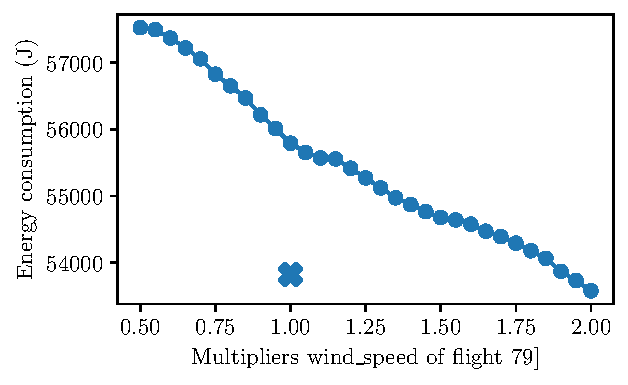
\includegraphics[width=0.9\linewidth]{figures/energy_vs_wind_speed.pdf}
    \caption{Energy consumption as a function of wind speed.}
    \label{fig:energy_vs_wind}
\end{figure}

Figure \ref{fig:energy_vs_wind} presents the predicted total energy consumption
as a function of the wind speed multiplier. The crossed marker at a multiplier of 1.0 indicates the baseline energy consumption corresponding to the measured power consumption. The observed trend shows a decrease in energy consumption with increasing wind speed, which initially appears counterintuitive. However, further analysis revealed that the wind was coming from behind the drone (tailwind), reducing aerodynamic drag and aiding forward motion. As a result, the UAV required less power, leading to lower energy consumption as wind speed increased.

\subsection{Effect of payload on energy consumption}
\begin{figure} [tph]
    \centering
    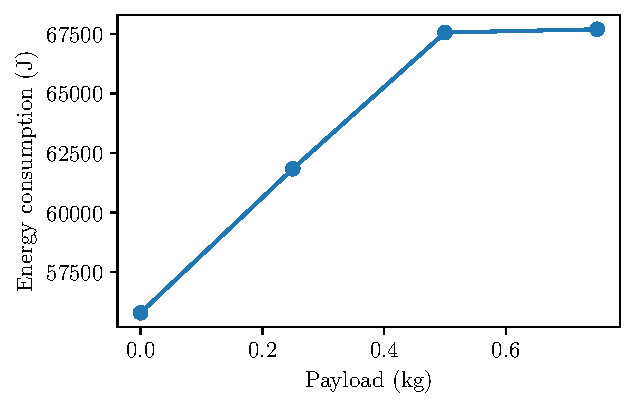
\includegraphics[width=0.9\linewidth]{figures/Energy_vs_payload.pdf}
    \caption{Energy consumption as a function of payload.}
    \label{fig:energy_vs_payload}
\end{figure}

To analyze the impact of payload on energy consumption, the payload mass is systematically varied while keeping all other flight parameters unchanged. 
Figure \ref{fig:energy_vs_payload} illustrates the relationship between payload mass and total energy consumption for Flight 79. The observed trend shows an increase in energy consumption with higher payload values, indicating the additional power required to sustain flight under increased mass. However, there is almost no observed increase in energy consumption when the payload is increased from 0.5 kg to 0.75 kg. This unexpected result is likely due to the limited training data available for the 0.75 kg payload. There are approximately 1,600 samples compared to around 80,000 samples for other payload levels i.e. 0 kg, 0.25 kg and 0.5 kg. As a result, the machine learning model’s ability to generalize and accurately predict energy behavior at 0.75 kg is significantly constrained, leading to unreliable predictions for this specific payload. 

\subsection{Effect of linear acceleration on energy consumption}
\begin{figure}[tph]
    \centering
    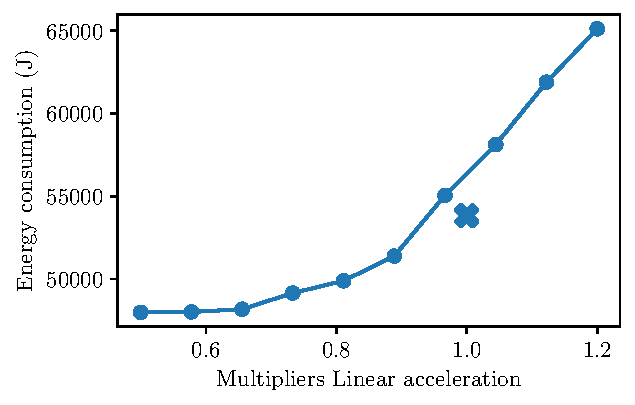
\includegraphics[width=0.9\linewidth]{figures/Energy_vs_az.pdf}
    \caption{Sensitivity of energy consumption to linear acceleration values in the training data range.}
    \label{fig:energy_vs_az}
\end{figure}

In addition to payload and wind effects, the influence of linear acceleration on energy consumption is evaluated to capture the impact of aggressive maneuvering and control effort. The linear acceleration components along the x, y, and z axes
of Flight 79 are scaled uniformly using multiplicative factors while keeping all other flight parameters unchanged. Figure \ref{fig:energy_vs_az} shows the variation in total energy consumption with increasing linear acceleration scaling. The increasing trend demonstrates that higher maneuvering intensity
leads to increased energy usage due to greater control effort and
propulsion demand.

\subsection{Feasibility analysis and return-to-home logic}
The predicted mission-level energy consumption obtained from the data-driven model enables a direct feasibility assessment for UAV operations. Using the sensitivity analyses presented in the previous sections, the effects of payload variation, wind speed scaling, and linear acceleration scaling on total mission energy consumption are quantified. Each scenario results in a modified energy estimate that represents the expected energy demand if the same trajectory were flown under altered conditions. These predicted energy values can be compared against the available onboard battery energy to assess mission feasibility. The Return-to-Home (RTH) decision logic can be formulated by comparing the predicted remaining energy required to complete the mission with the remaining battery capacity. If the estimated energy demand exceeds the available energy margin, the mission is classified as infeasible, and an RTH command can be triggered to ensure safe operation. Conversely, if sufficient energy margin exists, the mission may continue as planned. This framework demonstrates how the developed energy prediction models can be directly applied at the application level to support real-time decision-making. By continuously updating energy estimates based on changing payload, environmental conditions, and maneuver intensity, the UAV can autonomously assess mission feasibility and initiate safety actions when required.
